\documentclass[12pt,a4paper]{article}
\usepackage[utf8]{inputenc}
\usepackage[english,russian]{babel}
\usepackage[left=1cm,right=1cm,top=2cm,bottom=2cm,bindingoffset=0cm]{geometry} 
\usepackage{textcomp,latexsym,pb-diagram,amsopn} 
\usepackage{amsmath}
\usepackage{amsfonts}
\usepackage{amssymb}
\usepackage{makeidx}
\usepackage{amsmath}
\usepackage{amsfonts}
\usepackage{amssymb}
\usepackage{pdfpages}
\usepackage{cite,enumerate,float,indentfirst} 
\usepackage{graphicx,xcolor} 
\usepackage{float}
\usepackage{gnuplottex}
\usepackage{caption,setspace}
\captionsetup{font={small}}

\begin{document}
\title{Численное моделирование нестационарного течения газа с 
использованием разностной несимметричной схемы $Ln(p)$-СКОРОСТЬ}
\author{Бекбулатов Рамзан \\ 410 группа }

\maketitle

\section{\LARGE Тесты}

\subsection{ \Large Случай гладкого решения}
Проверка работоспособности схемы производилась для следующего гладкого решения:

\begin{figure}[h]
\center{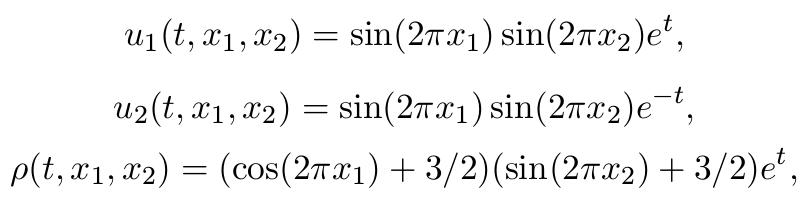
\includegraphics[width=0.5\linewidth]{./images/22.png}}
\end{figure}



\section{\LARGE Постановка задачи}
Решение краевой задачи протекания газа через область $\Omega$

Система уравнений, описывающая нестационарное движение баротропного газа в области $\Omega$ размерности 2 или 3, выглядит следующим образом

\begin{figure}[h]
\center{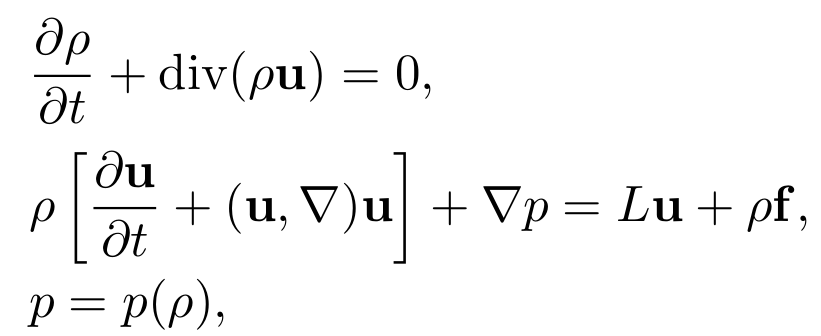
\includegraphics[width=0.4\linewidth]{./images/1.png}}
\end{figure}
где $L$ есть линейный симметричный положительно определенный оператор
\begin{figure}[h!]
\center{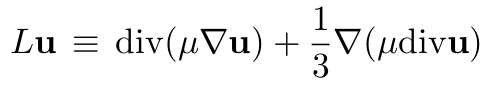
\includegraphics[width=0.35\linewidth]{./images/11.png}}
\end{figure}

Для построения разностной схемы в двумерном случае с односторонними разностями, направленными против потока, и вычисляемой функцией $g = ln(p)$ запишем систему в виде
\begin{figure}[h!]
\center{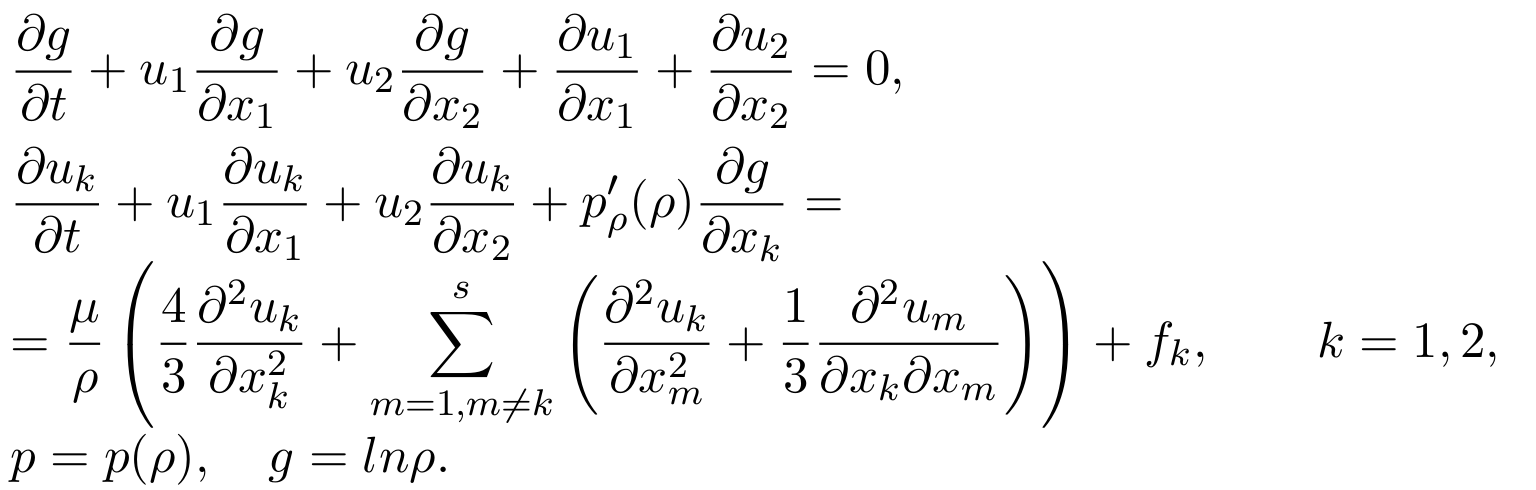
\includegraphics[width=0.8\linewidth]{./images/4.png}}
\end{figure}
\newpage
Неизвестные функции: плотность $p$ и вектор скорости $u$ являются функциями переменных Эйлера
\begin{figure}[h!] 
\center{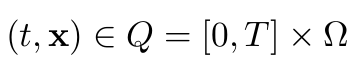
\includegraphics[width=0.27\linewidth]{./images/14.png}}
\end{figure}

В начальный момент времени задаются функции, значения которых определяют плотность и скорость газав каждой точке области $\Omega$:
\begin{figure}[h]
\center{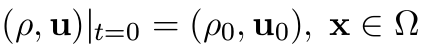
\includegraphics[width=0.3\linewidth]{./images/15.png}}
\end{figure}

\section{Область и граничные условия}
Компоненты функции скорости на границе области $\Omega$ будем считать равными нулю, если явно не задано другое условие. На границе, где вектор скорости направлен во внутрь, будем считать известной фукнцию плотности, положив её значение равным $\rho_{\gamma}$. На остальных участках границы функция плотности считается неизвестной и подлежит определению.

Обозначим через $\Omega_{nm}$ квадрат, координаты точек которого удовлетворяют неравенствам $n < x < n + 1$ и $m < y < m + 1$. Множества точек, составляюзие стороны квадрата $\Omega_{nm}$ обозначим $\Gamma^{x-}_{nm}$, $\Gamma^{x+}_{nm}$, $\Gamma^{y-}_{nm}$ и $\Gamma^{y+}_{nm}$, где индекс x или y означает, какая из координат на стороне является постоянной, а + или - означает максимальное или минимальное значение, которое принимает эта координата. С учетом этих обозначений область и начальные условия можно записать в следующем виде:
\begin{equation*}
\bar{\Omega} = \bar{\Omega}_{01}\cup\bar{\Omega}_{02}\cup\bar{\Omega}_{11}\cup\bar{\Omega}_{12}\cup\bar{\Omega}_{20}\cup\bar{\Omega}_{21}\cup\bar{\Omega}_{22};
\end{equation*}
\begin{equation*}
u_1(x, y) = w, \quad where \quad (x, y)\in \Gamma^{x-}_{01}\cup\Gamma^{x+}_{02};
\end{equation*}
\begin{equation*}
\dfrac{\partial u_2 (x, y)}{\partial y} = 0, \quad where \quad (x, y)\in \Gamma^{y-}_{20}
\end{equation*}



\section{\LARGE Алгоритм}

Используемые обозначения:
\begin{figure}[h!]
\center{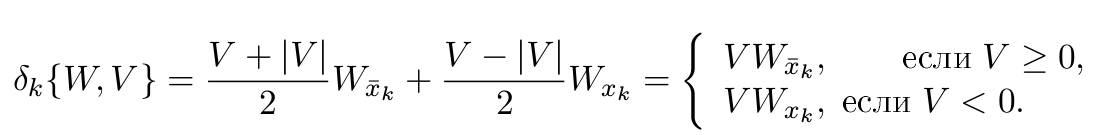
\includegraphics[width=0.6\linewidth]{./images/17.png}}
\center{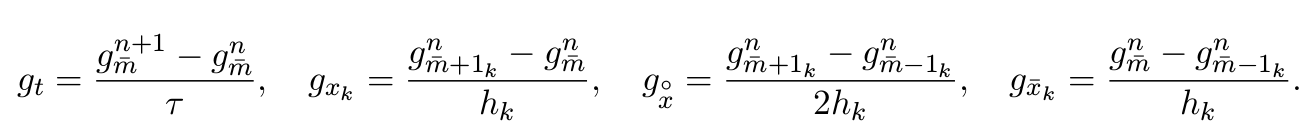
\includegraphics[width=0.8\linewidth]{./images/18.png}}
\end{figure} \\
Для поиска численного решения задачи предлагается использовать р.с.:
\begin{figure}[h!]
\center{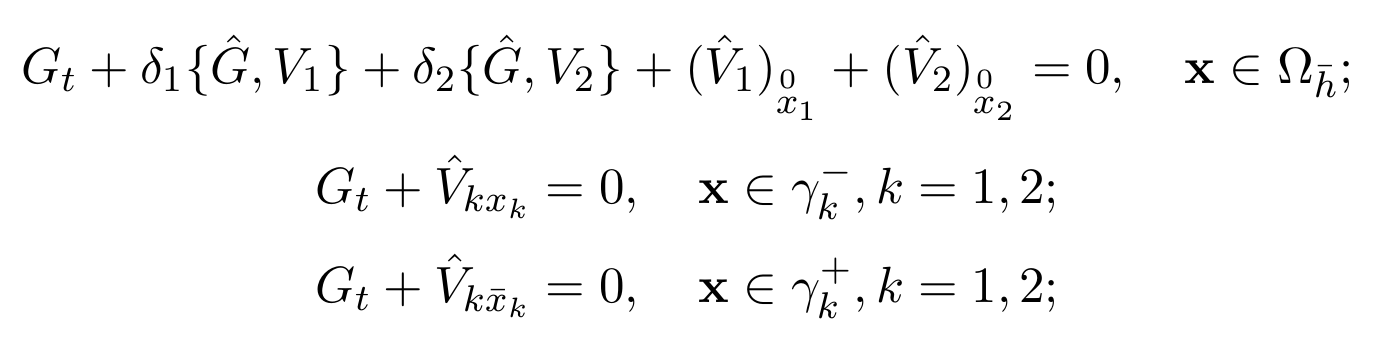
\includegraphics[width=0.6\linewidth]{./images/7.png}}
\center{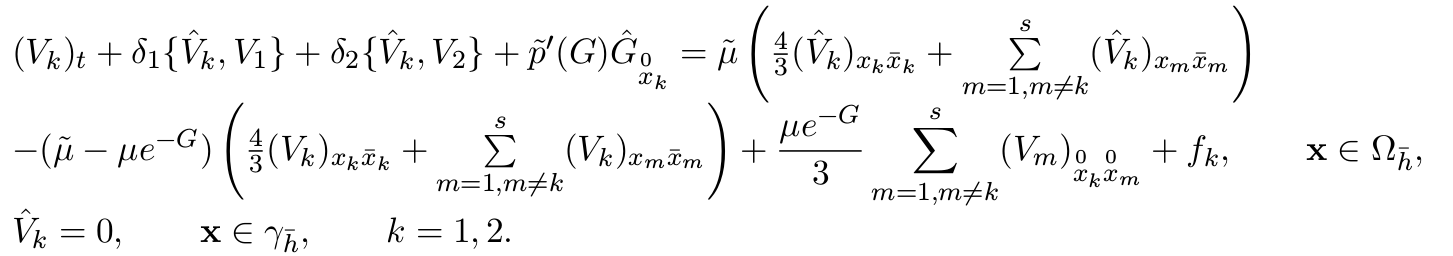
\includegraphics[width=0.9\linewidth]{./images/8.png}}
\end{figure} 
\begin{figure}[h!]
\center{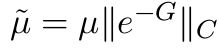
\includegraphics[width=0.16\linewidth]{./images/9.png}}
\end{figure} \\
\newpage
Приведем индексную запись уравнений данной разностной схемы:
\begin{figure}[h!]
\center{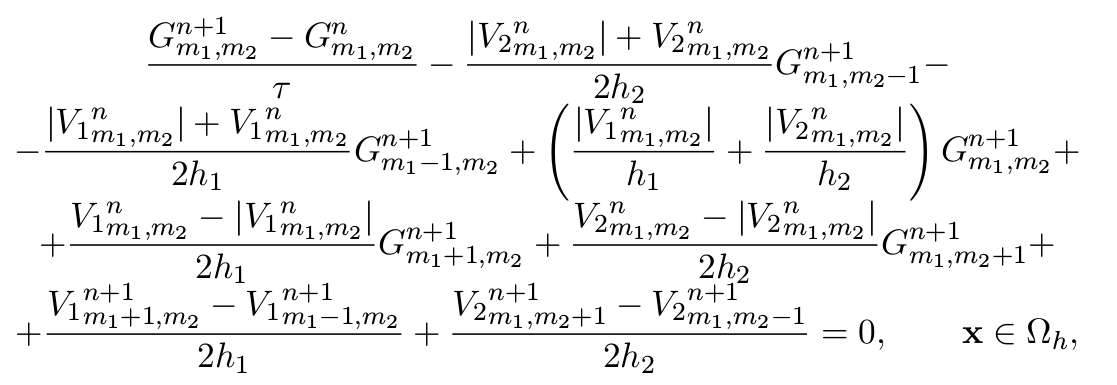
\includegraphics[width=0.75\linewidth]{./images/2.png}}
\end{figure}
\begin{figure}[h!]
\center{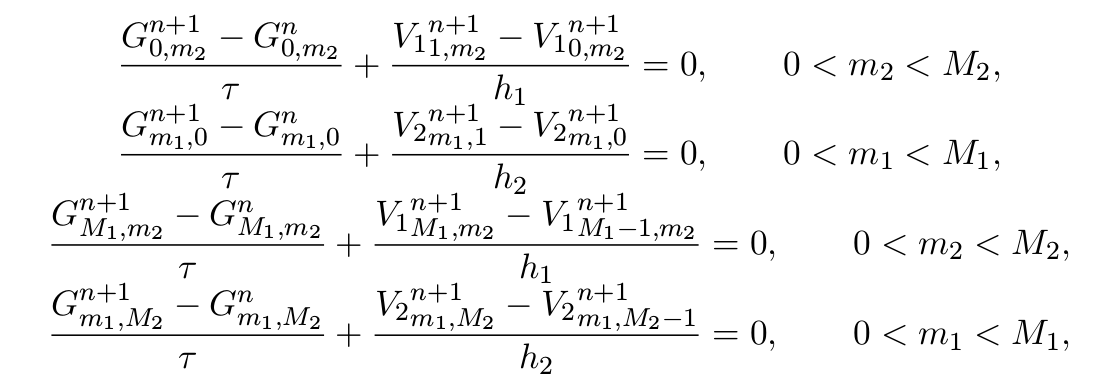
\includegraphics[width=0.75\linewidth]{./images/3.png}}
\end{figure}
\begin{figure}[h!]
\center{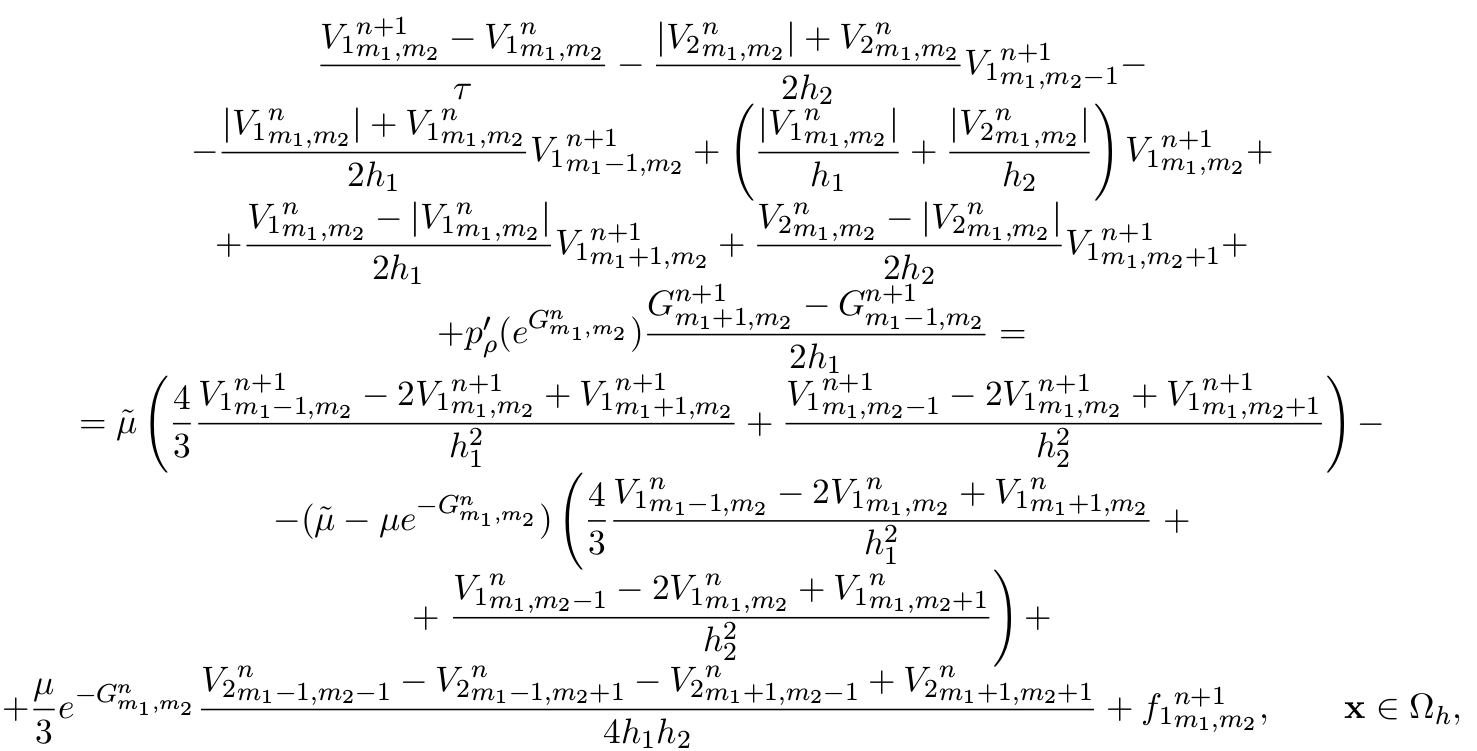
\includegraphics[width=0.95\linewidth]{./images/19.png}}
\end{figure}
\newpage
\begin{figure}[h!]
\center{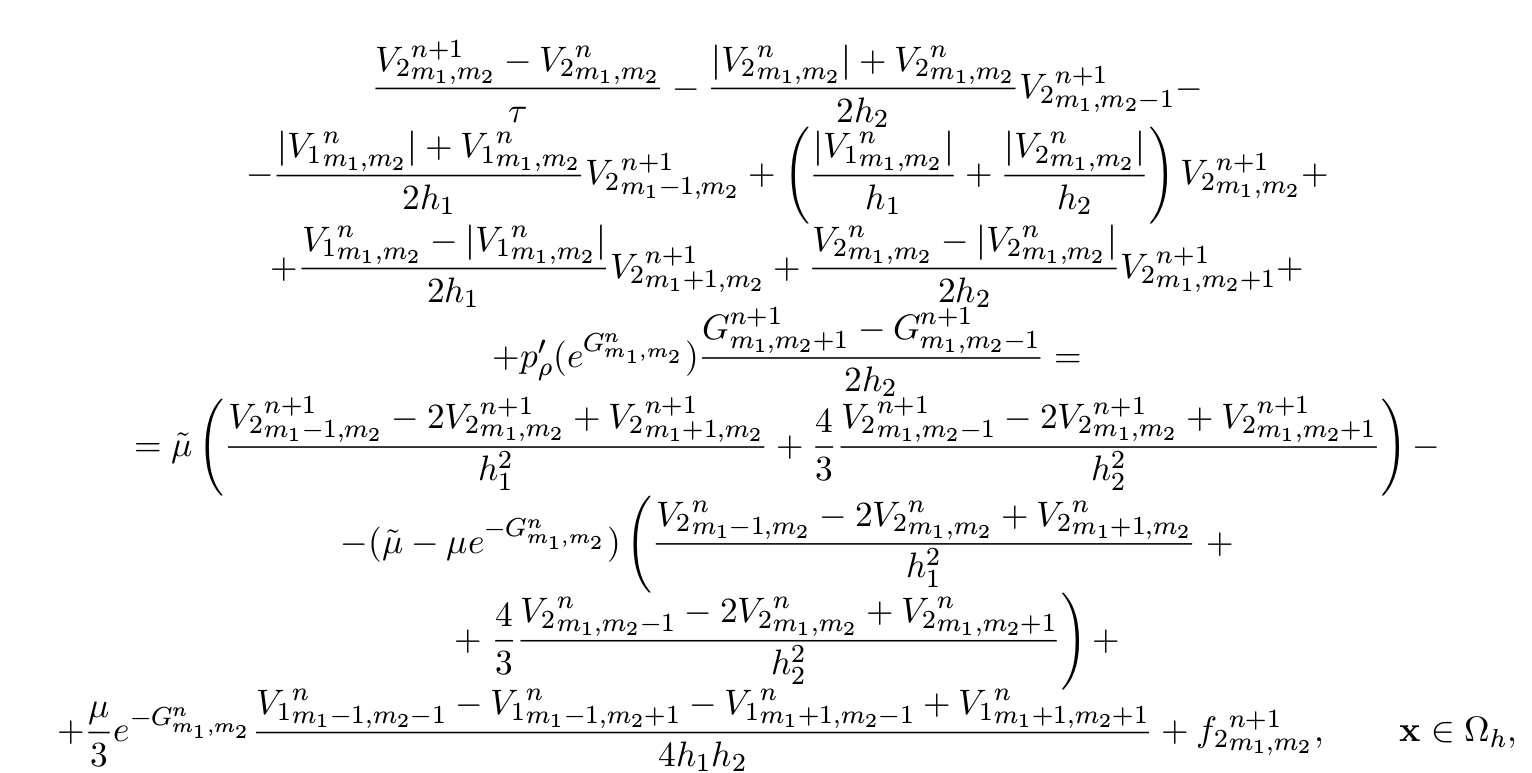
\includegraphics[width=0.95\linewidth]{./images/5.png}}
\end{figure} 
Данные уравнения образуют СЛАУ, решая которую находим сеточное решение на очередном слое.

Из первого разностного уравнения получаем следующие алгебраические уравнения для всех внутренних узлов:
\begin{figure}[h!]
{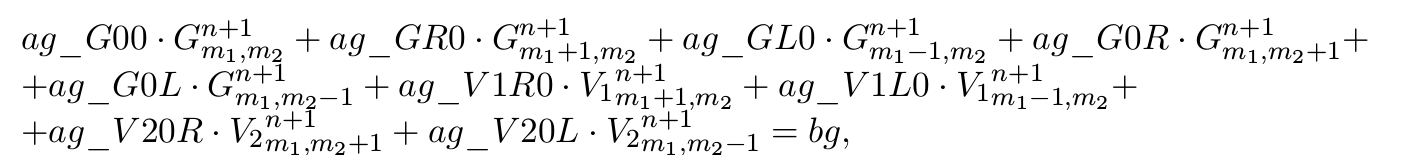
\includegraphics[width=0.93\linewidth]{./images/6.png}}
\end{figure} \\
где коэффициенты определяются по формулам:
\begin{figure}[h!]
{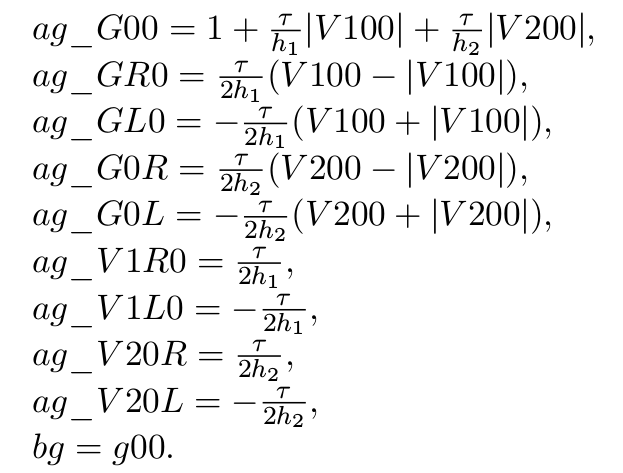
\includegraphics[width=0.38\linewidth]{./images/20.png}}
\end{figure} \\
Из третьего уравнения получаем: \\ \\
$ av1\_V100 \cdot (V_1)_{m_1,m_2}^{n+1} + av1\_V1R0 \cdot (V_1)_{m_1+1,m_2}^{n+1}
+ av1\_V1L0 \cdot (V_1)_{m_1-1,m_2}^{n+1} + av1\_V10R \cdot (V_1)_{m_1,m_2+1}^{n+1}
+ av1\_V10L \cdot (V_1)_{m_1,m_2-1}^{n+1} + av1\_GR0 \cdot G_{m_1 + 1,m_2}^{n+1}
+ av1\_GL0 * G_{m_1-1,m_2}^{n+1} = bv1,$ \\ \\
где \\ \\
$ av1\_V100 = 1 + \frac{\tau}{h_1}|V100| + \frac{\tau}{h_2}|V200| +  \tilde{\mu}\tau(\frac{8}{3h_1^2} + \frac{2}{h_2^2}) $ \\
$ av1\_V1L0 = -\frac{\tau}{2h_1}(|V100| + V100) - \frac{4\tilde \mu\tau}{3h_1^2} $ \\
$ av1\_V10L = -\frac{\tau}{2h_2}(|V200| + V200) - \frac{\tilde \mu\tau}  {h_2^2}  $ \\
$ av1\_V1R0 =  \frac{\tau}{2h_1}(V100 - |V100|) - \frac{4\tilde \mu\tau}{3h_1^2} $ \\
$ av1\_V10R =  \frac{\tau}{2h_2}(V200 - |V200|) - \frac{\tilde \mu\tau}  {h_2^2}  $ \\
$ av1\_GR0  =  \frac{\tau}{2h_1}\rho_p' $ \\
$ av1\_GL0  = -\frac{\tau}{2h_1}\rho_p' $
\begin{multline*}
bv1 = V100 + (-\tilde \mu + \mu e^{-g})(\frac{4\tau}{3h_1^2}(V1L0 - 2V1 + \\ +
  V1R0) + \frac{\tau}{h_2^2}(V10L - 2V1 + V10R)) +
  \\ + \frac{\mu\tau e^{-g}}{12h_1h_2}(V2LL - V2LR - V2RL + V2RR) + \tau F_{v2}
\end{multline*}
Из четвертого уравнения получаем: \\ \\
$ av2\_V200 \cdot (V_2)_{m_1,m_2}^{n+1} + av2\_V2R0 \cdot (V_2)_{m_1+1,m_2}^{n+1}
+ av2\_V2L0 \cdot (V_2)_{m_1-1,m_2}^{n+1} + av2\_V20R \cdot (V_2)_{m_1,m_2+1}^{n+1}
+ av2\_V20L \cdot (V_2)_{m_1,m_2-1}^{n+1} + av2\_GR0 \cdot G_{m_1 + 1,m_2}^{n+1}
+ av2\_GL0 * G_{m_1-1,m_2}^{n+1} = bv1,$ \\ \\
где \\ \\
$ av2\_V200 = 1 + \frac{\tau}{h_1}|V100| + \frac{\tau}{h_2}|V200| +  \tilde{\mu}\tau(\frac{8}{3h_2^2} + \frac{2}{h_1^2})$ \\
$ av2\_V2L0 = -\frac{\tau}{2h_1}(|V100| + V100) - \frac{\tilde \mu\tau}  {h_1^2}  $ \\
$ av2\_V20L = -\frac{\tau}{2h_2}(|V200| + V200) - \frac{4\tilde \mu\tau}{3h_2^2} $ \\
$ av2\_V2R0 =  \frac{\tau}{2h_1}(V100 - |V100|) - \frac{\tilde \mu\tau}  {h_1^2}  $ \\ 
$ av2\_V20R =  \frac{\tau}{2h_2}(V200 - |V200|) - \frac{4\tilde \mu\tau}{3h_2^2} $ \\
$ av2\_G0R  =  \frac{\tau}{2h_2}\rho_p'e^g $ \\
$ av2\_G0L  = -\frac{\tau}{2h_2}\rho_p'e^g $
\begin{multline*}
bv2 = V200 - (\tilde \mu - \mu e^{-g})(\frac{\tau}{h_1^2}(V2L0 - 2V2 +
\\ + V2R0) + \frac{4\tau}{3h_2^2}(V20L - 2V2 + V20R)) +
\\ + \frac{\mu\tau e^{-g}}{12h_1h_2}(V1LL - V1LR - V1RL + V1RR) + \tau F_{v2}
\end{multline*}

\section{Результаты расчета для гладкого решения}

Ниже представлена таблица точности расчетов для разных сеток. Из данных результатов следует, что точность вычислений 
возрастает при размельчении сетки.

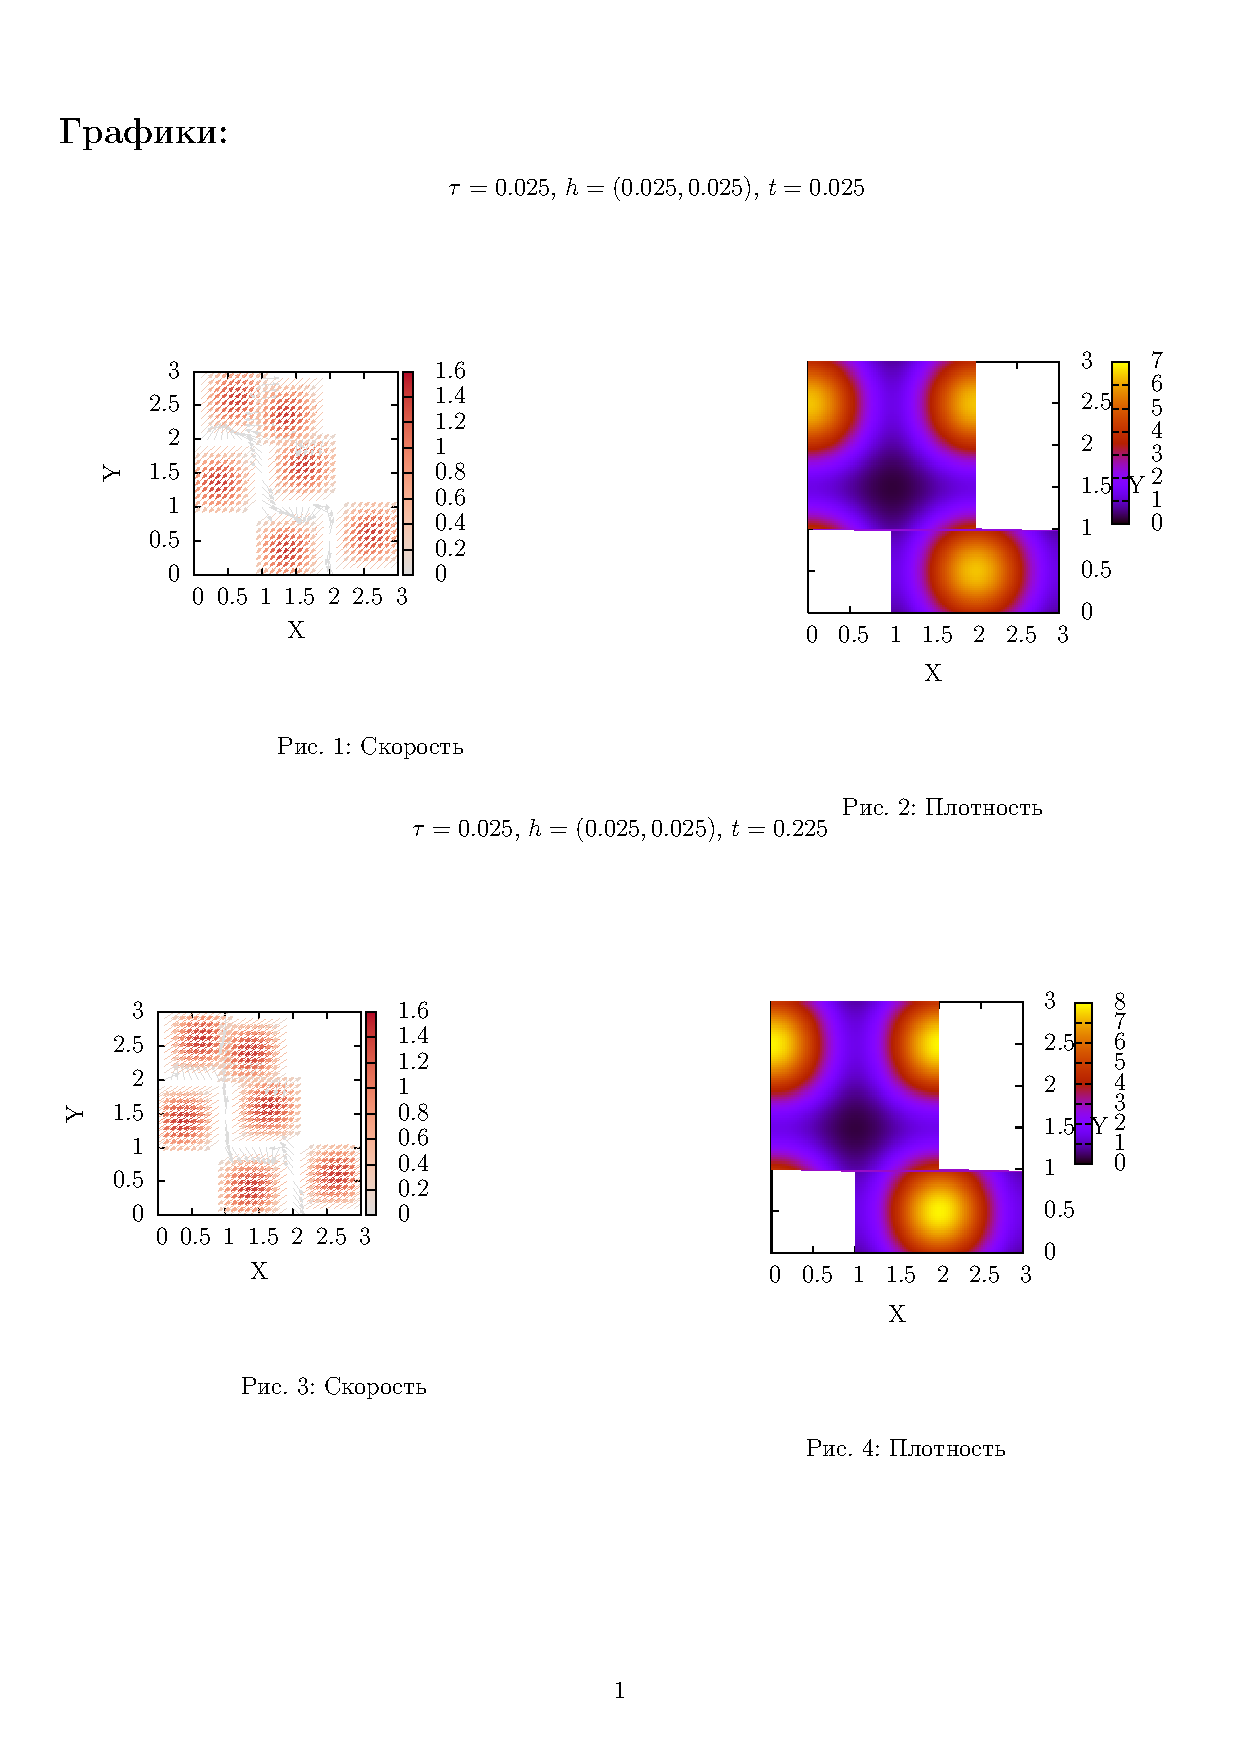
\includepdf[pages={-}]{plot_smooth.pdf}

 $norm\;of\;the\;error\;in\;C\;for\;g: \quad p_{\rho}=1.000, \mu = 0.100 \\ $
\begin{tabular}{|p{0.6in}|p{1.2in}|p{1.2in}|p{1.2in}|} \hline
$\tau\setminus h$ & $0.05000 $ & 0.02500 & 0.01250 \\ \hline
$0.05000$ & $9.908e-01$ &$6.824e-01$ &$5.356e-01$  \\ \hline
$0.02500$ & $8.234e-01$ &$4.873e-01$ &$3.289e-01$  \\ \hline
$0.01250$ & $7.447e-01$ &$4.048e-01$ &$2.403e-01$  \\ \hline
\end{tabular}\\[20pt]
  
$
 \text{norm of the error in $L_2$ for g}: \quad p_{\rho}=1.000, \mu = 0.100 \\ $
\begin{tabular}{|p{0.6in}|p{1.2in}|p{1.2in}|p{1.2in}|} \hline
$\tau\setminus h$ & $0.05000$ & $0.02500$& $0.01250$ \\ \hline
$0.05000$ & $1.840e-01$ &$1.263e-01$ &$1.007e-01$  \\ \hline
$0.02500$ & $1.482e-01$ &$8.847e-02$ &$6.119e-02$  \\ \hline
$0.01250$ & $1.321e-01$ &$7.177e-02$ &$4.345e-02$  \\ \hline
\end{tabular}\\[20pt]
 

 $norm\;of\;the\;error\;in\;C\;for\;v1: \quad p_{\rho}=1.000, \mu = 0.100 $ \\ 
\begin{tabular}{|p{0.6in}|p{1.2in}|p{1.2in}|p{1.2in}|} \hline
$\tau\setminus h$ & $0.05000 $ & 0.02500 & 0.01250 \\ \hline
$0.05000$ & $4.664e-01$ &$3.455e-01$ &$2.847e-01$  \\ \hline
$0.02500$ & $4.361e-01$ &$2.800e-01$ &$1.969e-01$  \\ \hline
$0.01250$ & $4.255e-01$ &$2.570e-01$ &$1.558e-01$  \\ \hline
\end{tabular}\\[20pt]
  

 $norm\;of\;the\;error\;in\;L_2\;for\;v1: \quad p_{\rho}=1.000, \mu = 0.100 $ \\ 
\begin{tabular}{|p{0.6in}|p{1.2in}|p{1.2in}|p{1.2in}|} \hline
$\tau\setminus h$ & $0.05000 $ & 0.02500 & 0.01250 \\ \hline
$0.05000$ & $1.374e-01$ &$9.638e-02$ &$7.556e-02$  \\ \hline
$0.02500$ & $1.275e-01$ &$7.925e-02$ &$5.293e-02$  \\ \hline
$0.01250$ & $1.247e-01$ &$7.271e-02$ &$4.298e-02$  \\ \hline
\end{tabular}\\[20pt]
 
\newpage

 $norm\;of\;the\;error\;in\;C\;for\;v2: \quad p_{\rho}=1.000, \mu = 0.100 $ \\ 
\begin{tabular}{|p{0.6in}|p{1.2in}|p{1.2in}|p{1.2in}|} \hline
$\tau\setminus h$ & $0.05000 $ & 0.02500 & 0.01250 \\ \hline
$0.05000$ & $2.871e-01$ &$1.967e-01$ &$1.564e-01$  \\ \hline
$0.02500$ & $2.492e-01$ &$1.519e-01$ &$1.022e-01$  \\ \hline
$0.01250$ & $2.277e-01$ &$1.297e-01$ &$7.782e-02$  \\ \hline
\end{tabular}\\[20pt]
  

 $norm\;of\;the\;error\;in\;L_2\;for\;v2: \quad p_{\rho}=1.000, \mu = 0.100 $ \\ 
\begin{tabular}{|p{0.6in}|p{1.2in}|p{1.2in}|p{1.2in}|} \hline
$\tau\setminus h$ & $0.05000 $ & 0.02500 & 0.01250 \\ \hline
$0.05000$ & $9.131e-02$ &$6.581e-02$ &$5.306e-02$  \\ \hline
$0.02500$ & $7.585e-02$ &$4.852e-02$ &$3.433e-02$  \\ \hline
$0.01250$ & $6.821e-02$ &$4.009e-02$ &$2.508e-02$  \\ \hline
\end{tabular}\\[20pt]
 

 $ time, p_{\rho}=1.000, \mu = 0.100 $ \\ 
\begin{tabular}{|p{0.6in}|p{1.2in}|p{1.2in}|p{1.2in}|} \hline
$\tau\setminus h$ & $0.05000 $ & 0.02500 & 0.01250 \\ \hline
$0.05000$ & $7.056e-01$ &$4.954e+00$ &$4.219e+01$  \\ \hline
$0.02500$ & $1.091e+00$ &$6.653e+00$ &$4.727e+01$  \\ \hline
$0.01250$ & $1.772e+00$ &$1.036e+01$ &$6.161e+01$  \\ \hline
\end{tabular}\\[20pt]
 


\section{Результаты расчета задачи протекания}
После отладки схемы на гладком решении были проведен расчет задачи протекания при различных значения параметров $\rho_{\gamma}$ и $w$. Ниже представлены результаты.

\subsection{Графики при $\rho_{0} = 0.5, \rho_{\gamma} = 0.3, w = 0.1$}
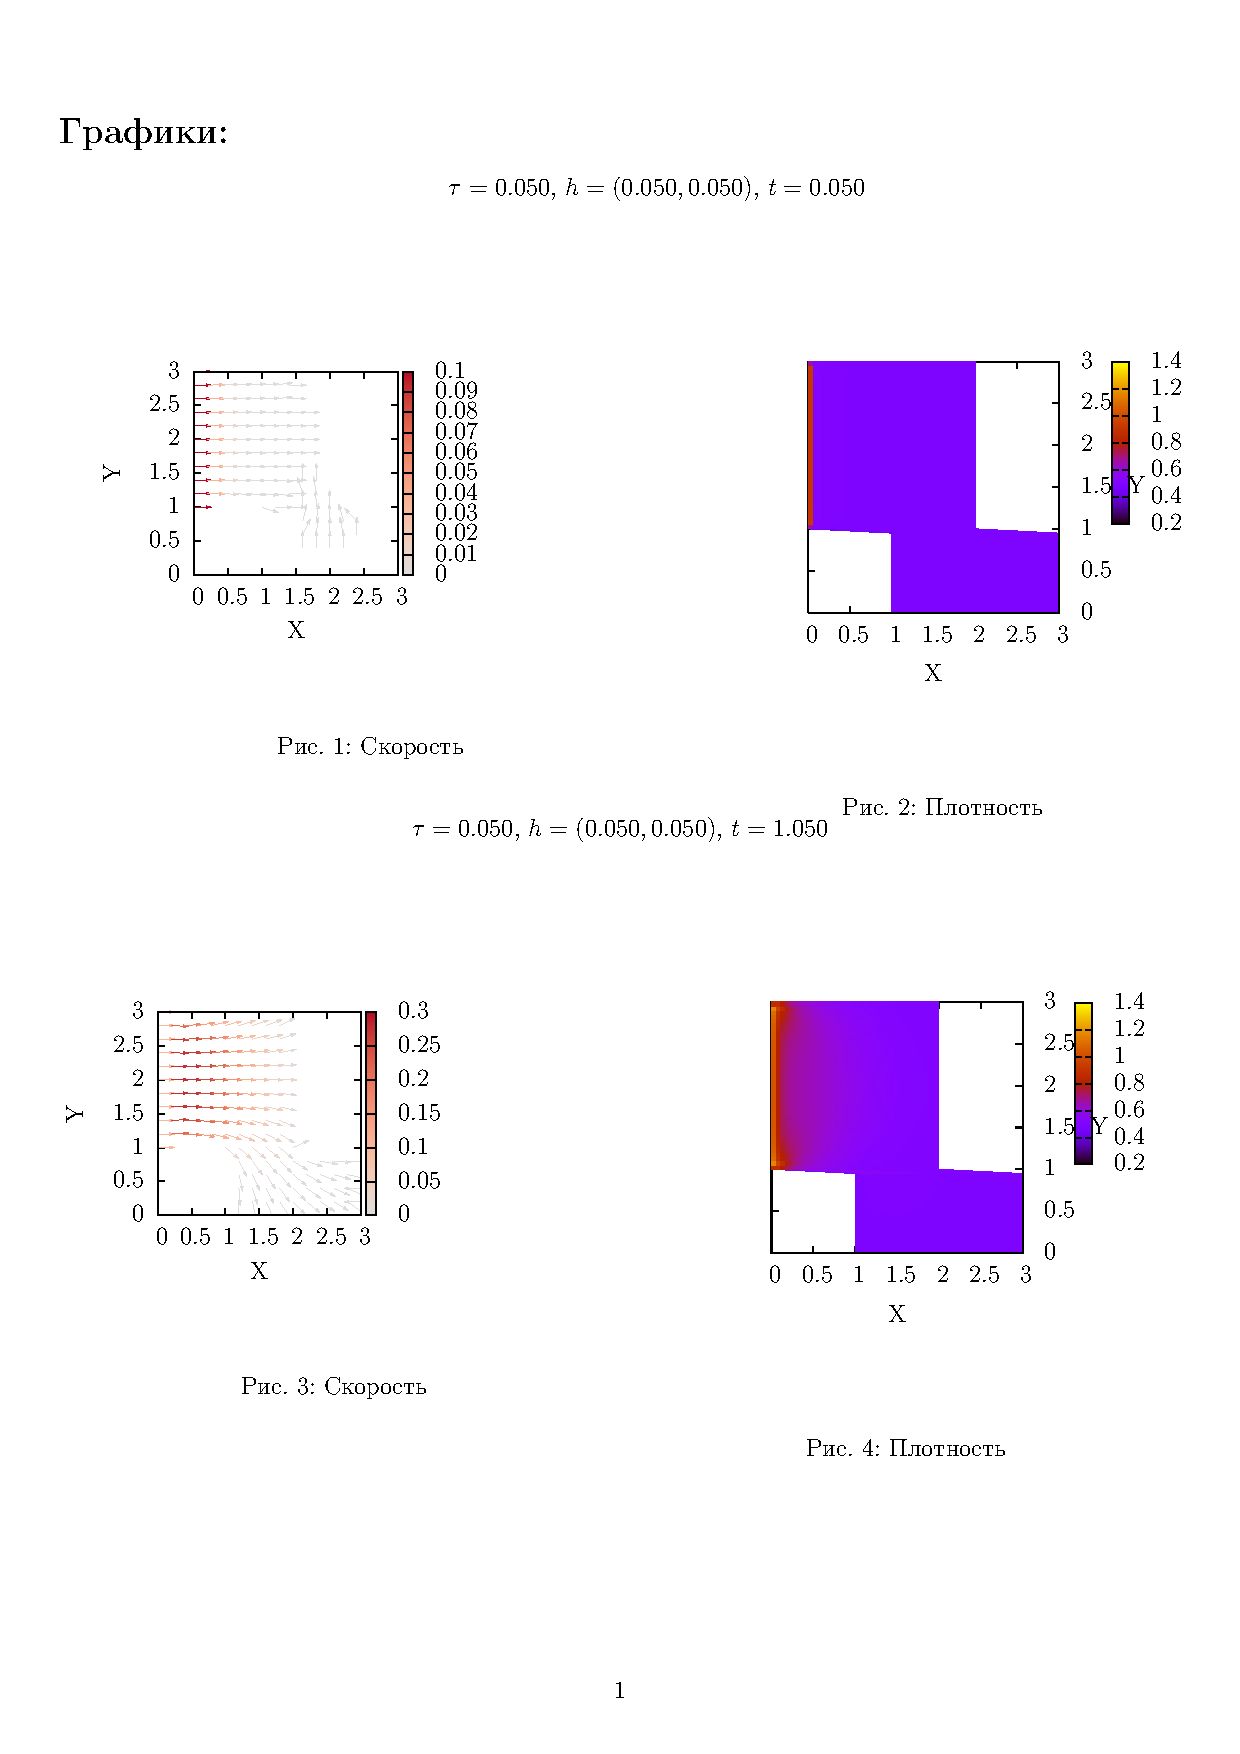
\includepdf[pages={-}]{plot_abrupt_5_3_1.pdf}

\subsection{Графики при $\rho_{0} = 0.5, \rho_{\gamma} = 0.3, w = 0.5$}
Эти графики отображают моделирование более быстрого втекания газа. \\
Видны небольшие ударные волны.
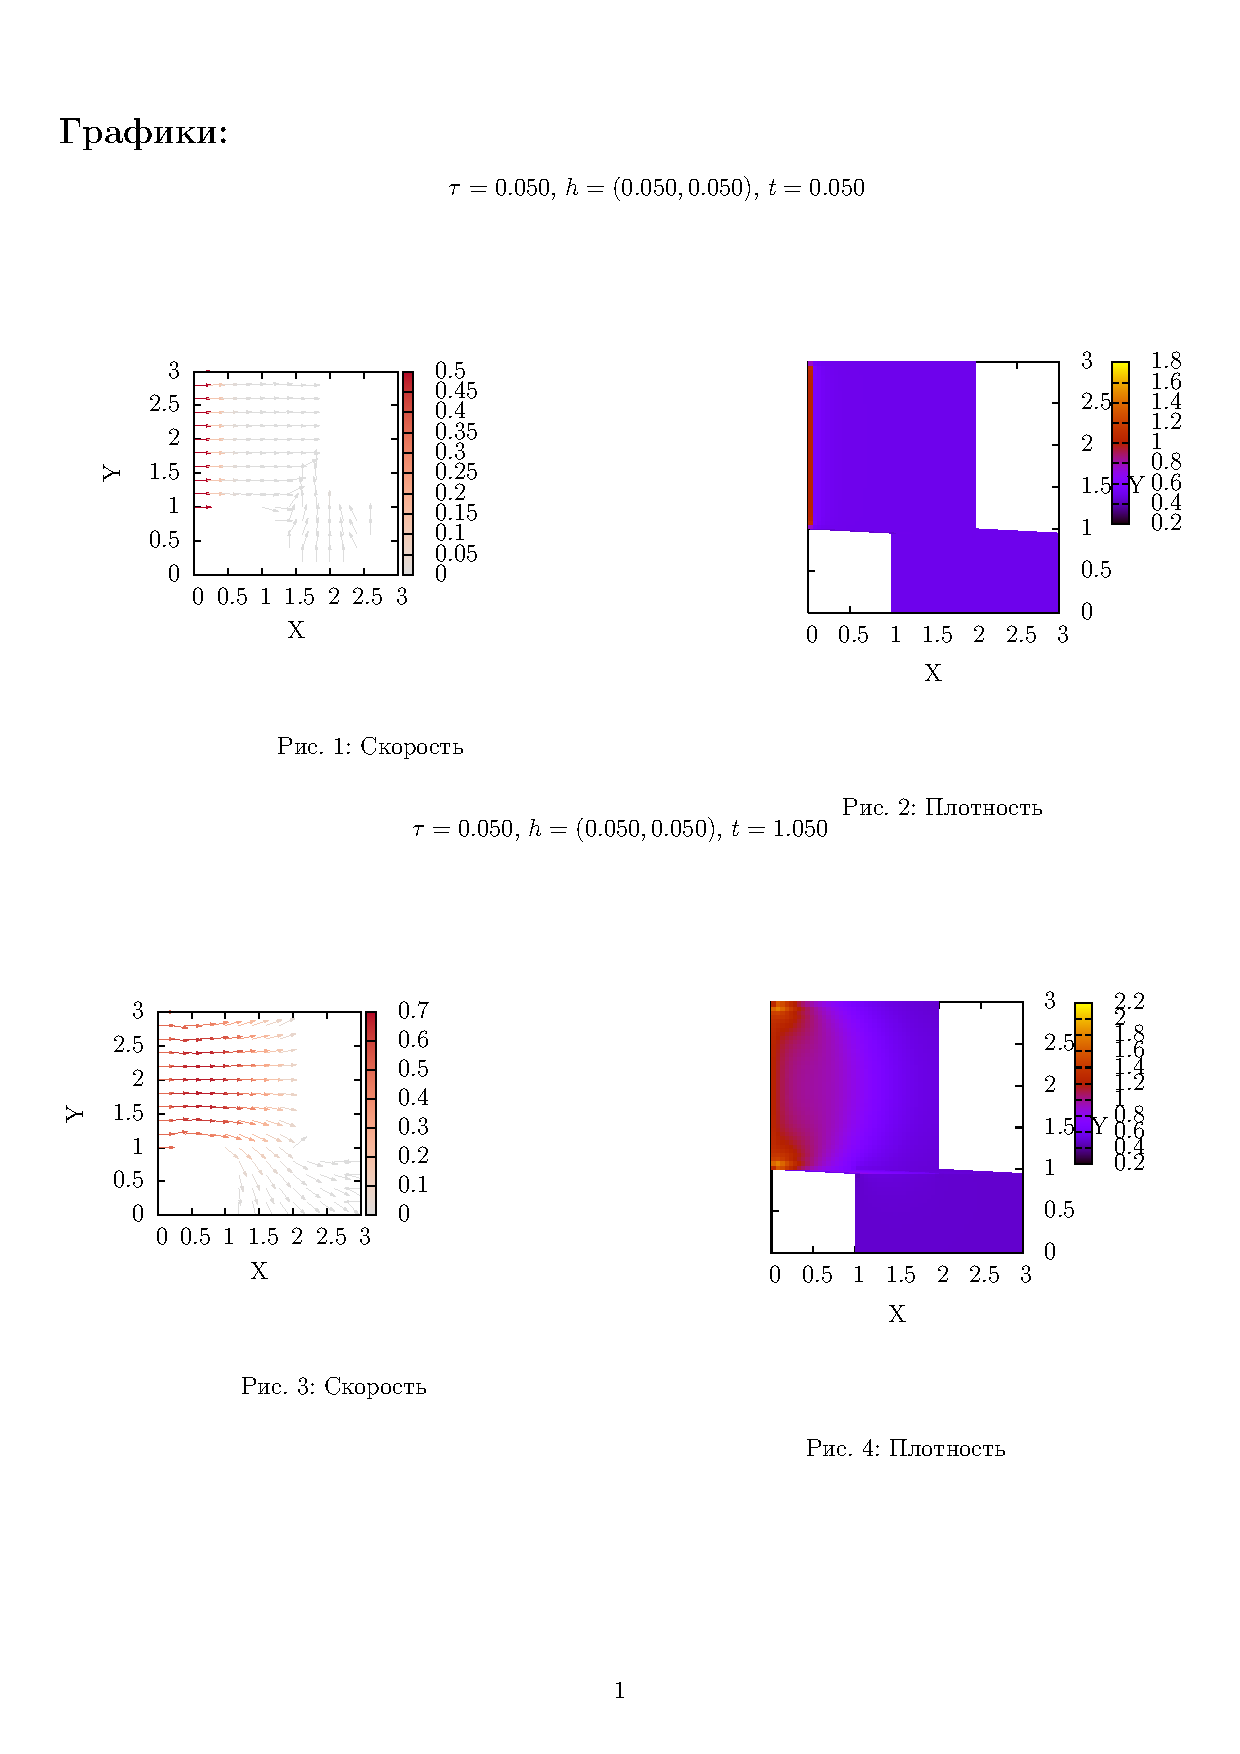
\includepdf[pages={-}]{plot_abrupt_5_3_5.pdf}

\subsection{Графики при $\rho_{0} = 0.5, \rho_{\gamma} = 0.3, w = 1.0$}
Эти графики отображают моделирование еще более быстрого втекания газа. \\
Видны сильные ударные волны и завихрения.
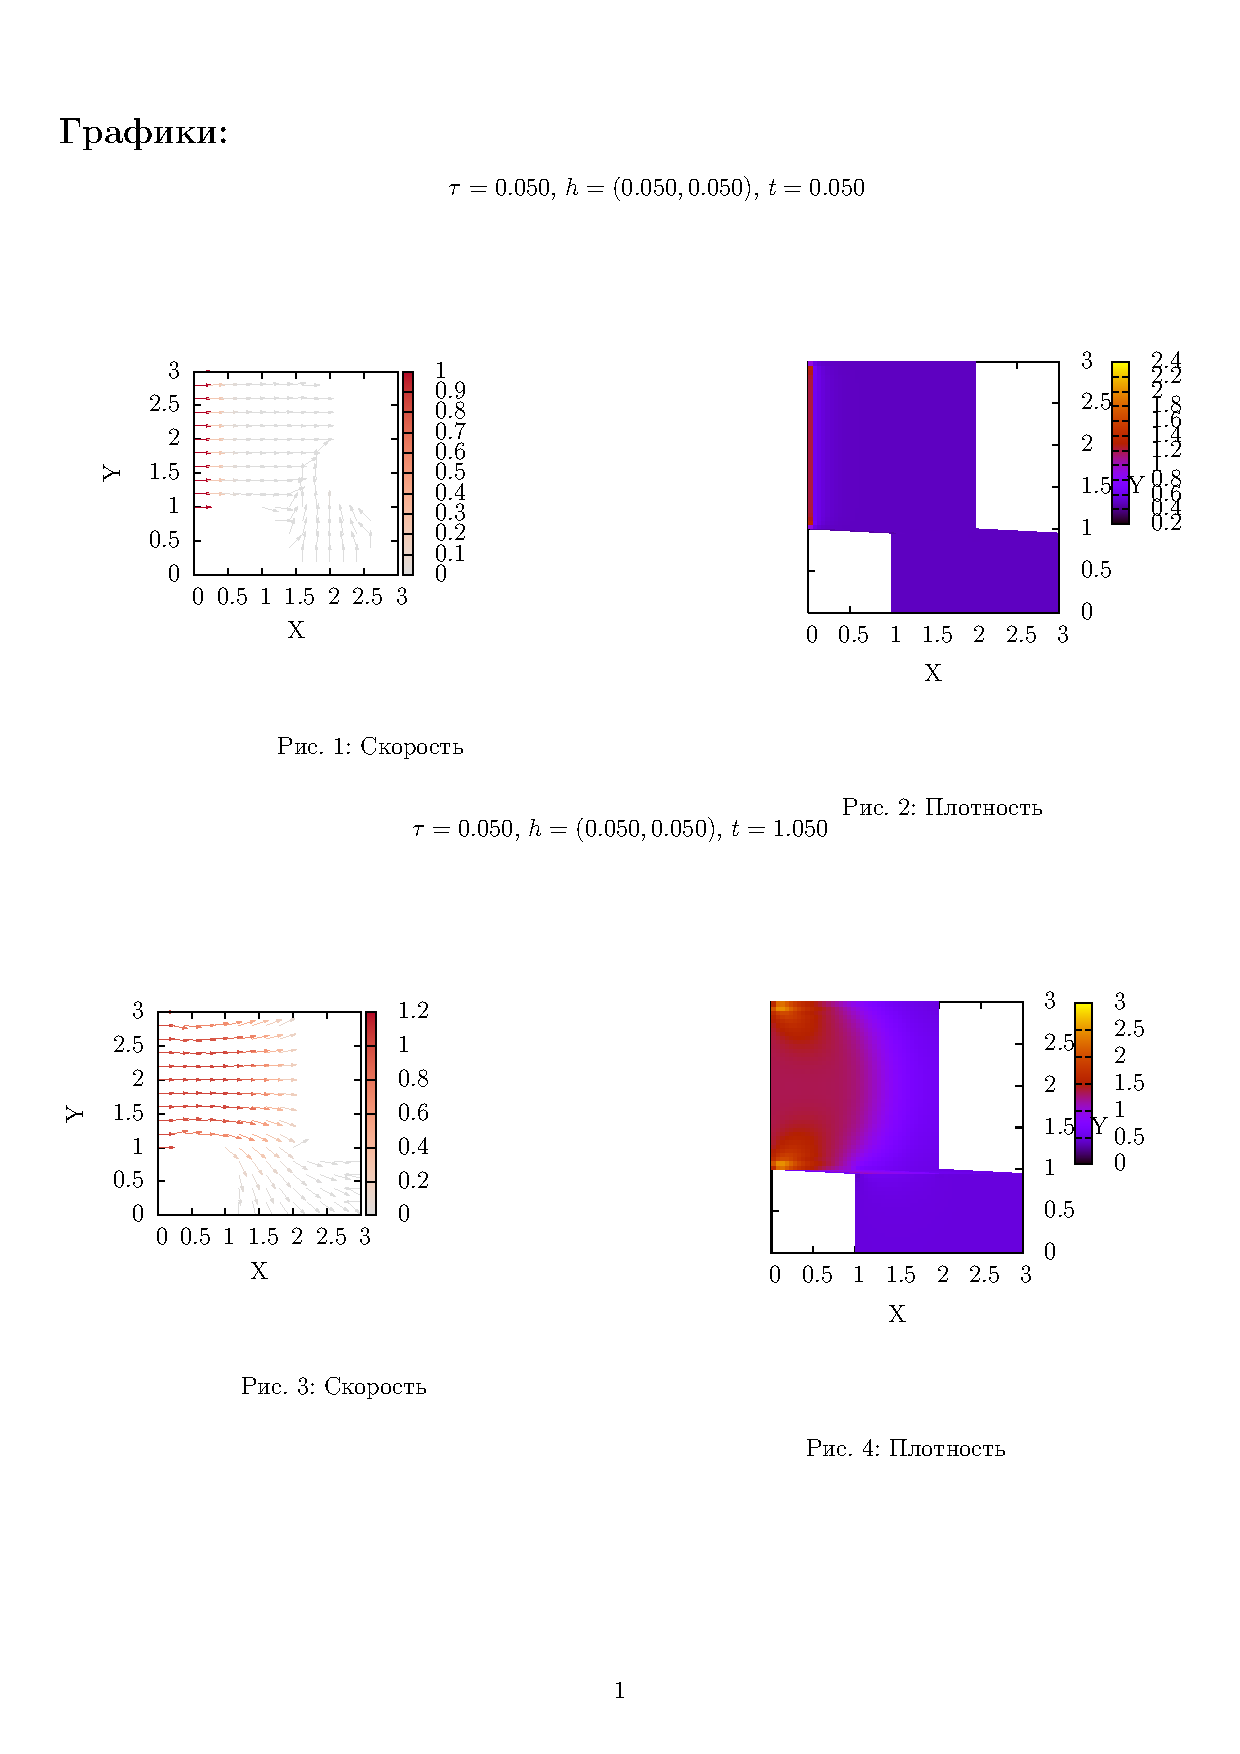
\includepdf[pages={-}]{plot_abrupt_5_3_10.pdf}

\subsection{Графики при $\rho_{0} = 0.1, \rho_{\gamma} = 0.5, w = 0.1$}
Эти графики отображают моделирование медленного втекания плотного газа в разреженную среду.
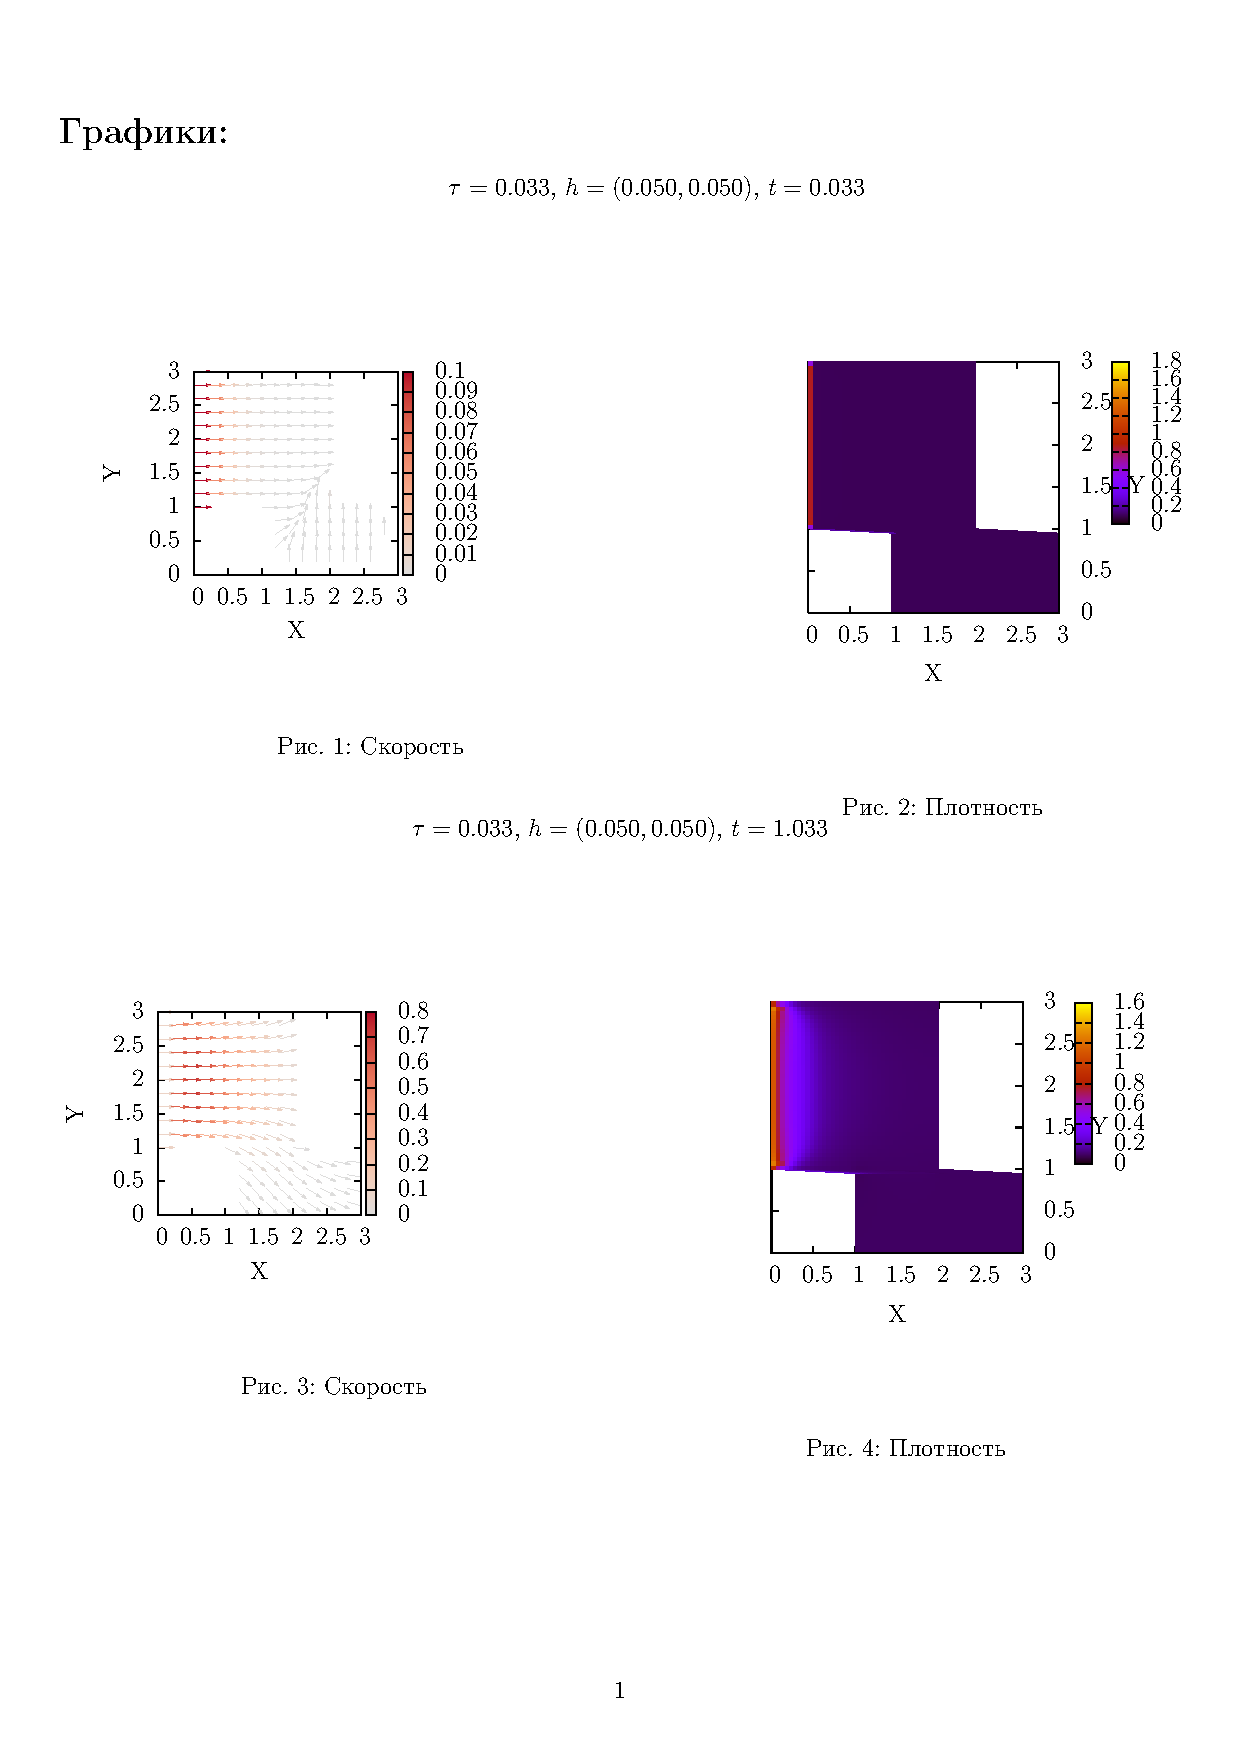
\includepdf[pages={-}]{plot_abrupt_1_5_1.pdf}

\section{Спектр линеризованного разностного оператора}
Стационарное решение было найдено следующим способом: на итерациях проверялась норма текущего решения по сравнению с предыдущим. Критерием выхода было выбрано значение $eps = 1.e-12$. Стационарное решение было найдено:
\begin{center}
N = 4000, M1 =  60, M2 =  60, Dim =   2521.                 \\
t =    1, norm = 1.072538e-01                               \\
t =  100, norm = 1.942510e-03                               \\
t =  200, norm = 9.581218e-04                               \\
t =  300, norm = 5.200315e-04                               \\
t =  400, norm = 2.968678e-04                               \\
t =  500, norm = 1.745928e-04                               \\
t =  600, norm = 1.046111e-04                               \\
t =  700, norm = 6.341809e-05                               \\
t =  800, norm = 3.872874e-05                               \\
t =  900, norm = 2.375964e-05                               \\
t = 1000, norm = 1.461777e-05                               \\
t = 1100, norm = 9.009206e-06                               \\
t = 1200, norm = 5.558587e-06                               \\
t = 1300, norm = 3.431910e-06                               \\
t = 1400, norm = 2.119779e-06                               \\
t = 1500, norm = 1.309666e-06                               \\
t = 1600, norm = 8.092901e-07                               \\
t = 1700, norm = 5.001458e-07                               \\
t = 1800, norm = 3.091189e-07                               \\
t = 1900, norm = 1.910678e-07                               \\
t = 2000, norm = 1.181082e-07                               \\
t = 2100, norm = 7.301506e-08                               \\
t = 2200, norm = 4.513974e-08                               \\
t = 2300, norm = 2.790872e-08                               \\
t = 2400, norm = 1.725944e-08                               \\
t = 2500, norm = 1.067561e-08                               \\
t = 2600, norm = 6.602656e-09                               \\
t = 2700, norm = 4.090830e-09                               \\
t = 2800, norm = 2.530869e-09                               \\
t = 2900, norm = 1.569131e-09                               \\
t = 3000, norm = 9.622032e-10                               \\
t = 3100, norm = 5.999068e-10                               \\
t = 3200, norm = 3.692501e-10                               \\
t = 3300, norm = 1.493756e-10                               \\
t = 3400, norm = 6.684053e-11                               \\
Stationary solution has been found at T = 3485.             \\
Current norm = 0.000000e+00, criteria norm = 1.000000e-12.  \\
Elapsed time: 30.28 sec.                                    \\
\end{center}
 
Рассмотрим линеризацию разностного оператора на стационарном решении:
\begin{figure}[h!]
\center{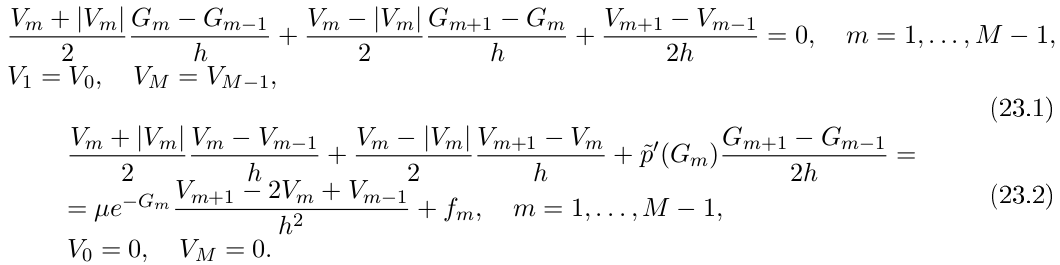
\includegraphics[width=0.8\linewidth]{./images/linear231.png}}
\end{figure}
\begin{figure}[h!]
\center{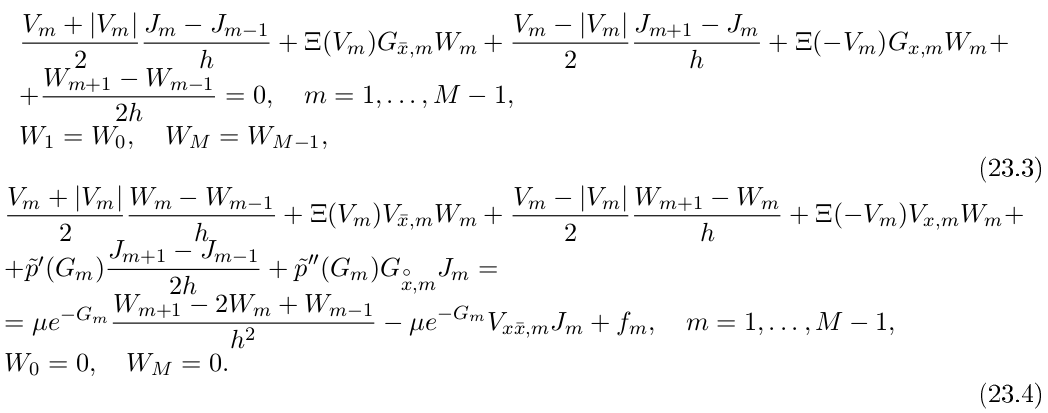
\includegraphics[width=0.8\linewidth]{./images/linear232.png}}
\end{figure}
\begin{figure}[h!]
\center{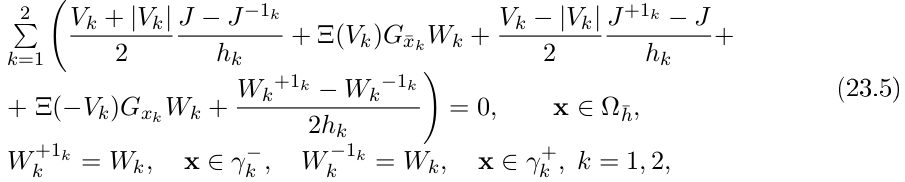
\includegraphics[width=0.8\linewidth]{./images/linear233.png}}
\end{figure}
\begin{figure}[h!]
\center{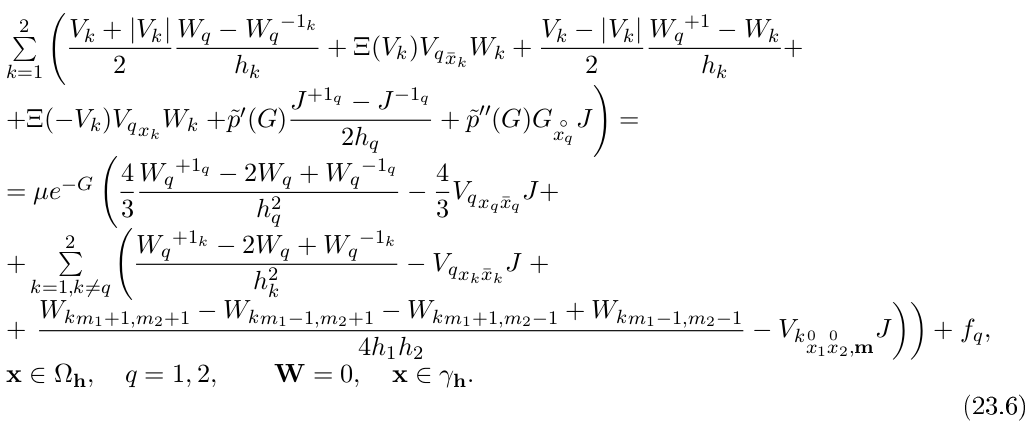
\includegraphics[width=0.8\linewidth]{./images/linear234.png}}
\end{figure}
\newpage

С помощью метода Арнольди было найдены собственные значения задачи. Приведем 6 значений с  максимальным модулем действительной части:
\begin{eqnarray*}
	Arnoldi iter =  166                                                 \\
	Arnoldi: found 6 vectors. Accuracy = 1.00e-12                       \\
	\lambda_1 = 3.50627e+02 + 0.00000e+00 * i, |\lambda| = 3.50627e+02  \\
	\lambda_2 = 3.48377e+02 + 0.00000e+00 * i, |\lambda| = 3.48377e+02  \\
	\lambda_3 = 3.47545e+02 + 0.00000e+00 * i, |\lambda| = 3.47545e+02  \\
	\lambda_4 = 3.45528e+02 + 0.00000e+00 * i, |\lambda| = 3.45528e+02  \\
	\lambda_5 = 3.39544e+02 + 0.00000e+00 * i, |\lambda| = 3.39544e+02  \\
	\lambda_6 = 3.39581e+02 + 0.00000e+00 * i, |\lambda| = 3.39581e+02
\end{eqnarray*}

Далее собственная функция, соответствующая $\lambda_1$, была добавлена к стационарному решению исходной задачи протекания для проверки стабилизации.

После применения первой собственной функции решение стабилизировалось:
\begin{center}
N = 4000, M1 =  60, M2 =  60, Dim =   2521.                  \\
t =   1, norm = 9.970386e-03                                 \\
t = 100, norm = 3.436912e-07                                 \\
t = 200, norm = 1.683891e-08                                 \\
t = 300, norm = 2.701169e-09                                 \\
t = 400, norm = 1.554984e-09                                 \\
t = 500, norm = 9.699501e-10                                 \\
t = 600, norm = 6.046833e-10                                 \\
t = 700, norm = 3.652314e-10                                 \\
t = 800, norm = 1.527191e-10                                 \\
t = 900, norm = 6.757690e-11                                 \\
Solution has stabilized at T = 986.                          \\
Current norm = 0.000000e+00, criteria norm = 1.000000e-12.   \\
Elapsed time: 11.79 sec.
\end{center}

Для второй собственной функции решение также стабилизировалось:
\begin{center}
N = 4000, M1 =  60, M2 =  60, Dim =   2521.                   \\
t =   1, norm = 1.088598e-02                                  \\
t = 100, norm = 3.720628e-07                                  \\
t = 200, norm = 5.040094e-08                                  \\
t = 300, norm = 3.130503e-08                                  \\
t = 400, norm = 1.910154e-08                                  \\
t = 500, norm = 1.182763e-08                                  \\
t = 600, norm = 7.313686e-09                                  \\
t = 700, norm = 4.531676e-09                                  \\
t = 800, norm = 2.804108e-09                                  \\
t = 900, norm = 1.738338e-09                                  \\
t = 1000, norm = 1.072804e-09                                 \\
t = 1100, norm = 6.631302e-10                                 \\
t = 1200, norm = 4.092234e-10                                 \\
t = 1300, norm = 1.994203e-10                                 \\
t = 1400, norm = 6.870039e-11                                 \\
t = 1500, norm = 5.923766e-11                                 \\
Solution has stabilized at T = 1509.                          \\
Current norm = 0.000000e+00, criteria norm = 1.000000e-12.    \\
Elapsed time: 17.01 sec.
\end{center}

Для третьей собственной функции решение также стабилизировалось:
\begin{center}
N = 4000, M1 =  60, M2 =  60, Dim =   2521.                   \\
t =   1, norm = 1.013349e-02                                  \\
t = 100, norm = 3.541050e-07                                  \\
t = 200, norm = 2.530480e-08                                  \\
t = 300, norm = 1.233945e-08                                  \\
t = 400, norm = 7.533702e-09                                  \\
t = 500, norm = 4.672422e-09                                  \\
t = 600, norm = 2.891578e-09                                  \\
t = 700, norm = 1.792497e-09                                  \\
t = 800, norm = 1.106697e-09                                  \\
t = 900, norm = 6.857592e-10                                  \\
t = 1000, norm = 4.242642e-10                                 \\
t = 1100, norm = 2.375473e-10                                 \\
t = 1200, norm = 7.015539e-11                                 \\
t = 1300, norm = 5.988882e-11                                 \\
Solution has stabilized at T = 1311.                          \\
Current norm = 0.000000e+00, criteria norm = 1.000000e-12.    \\
Elapsed time: 14.91 sec.
\end{center}


Для четвертой собственной функции решение также стабилизировалось:
\begin{center}
N = 4000, M1 =  60, M2 =  60, Dim =   2521.                    \\
t =   1, norm = 1.090894e-02                                   \\
t = 100, norm = 4.198660e-07                                   \\
t = 200, norm = 1.049851e-07                                   \\
t = 300, norm = 6.565253e-08                                   \\
t = 400, norm = 4.036074e-08                                   \\
t = 500, norm = 2.497339e-08                                   \\
t = 600, norm = 1.544643e-08                                   \\
t = 700, norm = 9.555498e-09                                   \\
t = 800, norm = 5.910908e-09                                   \\
t = 900, norm = 3.662350e-09                                   \\
t = 1000, norm = 2.266177e-09                                  \\
t = 1100, norm = 1.405104e-09                                  \\
t = 1200, norm = 8.623643e-10                                  \\
t = 1300, norm = 5.134168e-10                                  \\
t = 1400, norm = 3.215435e-10                                  \\
t = 1500, norm = 1.386173e-10                                  \\
t = 1600, norm = 6.424363e-11                                  \\
Solution has stabilized at T = 1661.                           \\
Current norm = 0.000000e+00, criteria norm = 1.000000e-12.     \\
Elapsed time: 18.55 sec.
\end{center}

Для пятой собственной функции решение также стабилизировалось:
\begin{center}
N = 4000, M1 =  60, M2 =  60, Dim =   2521.                     \\
t =   1, norm = 1.004870e-02                                    \\
t = 100, norm = 4.180139e-07                                    \\
t = 200, norm = 3.136801e-08                                    \\
t = 300, norm = 1.561810e-08                                    \\
t = 400, norm = 9.548538e-09                                    \\
t = 500, norm = 5.911163e-09                                    \\
t = 600, norm = 3.662483e-09                                    \\
t = 700, norm = 2.266674e-09                                    \\
t = 800, norm = 1.405395e-09                                    \\
t = 900, norm = 8.644294e-10                                    \\
t = 1000, norm = 5.346515e-10                                   \\
t = 1100, norm = 3.138216e-10                                   \\
t = 1200, norm = 1.432650e-10                                   \\
t = 1300, norm = 6.495314e-11                                   \\
Solution has stabilized at T = 1360.                            \\
Current norm = 0.000000e+00, criteria norm = 1.000000e-12.      \\
Elapsed time: 15.84 sec.
\end{center}

Для шестой собственной функции решение также стабилизировалось:
\begin{center}
N = 4000, M1 =  60, M2 =  60, Dim =   2521.                      \\
t =   1, norm = 1.065324e-02                                     \\
t = 100, norm = 3.669774e-07                                     \\
t = 200, norm = 1.868236e-08                                     \\
t = 300, norm = 3.605582e-09                                     \\
t = 400, norm = 1.782717e-09                                     \\
t = 500, norm = 1.119974e-09                                     \\
t = 600, norm = 6.984032e-10                                     \\
t = 700, norm = 4.271692e-10                                     \\
t = 800, norm = 2.427541e-10                                     \\
t = 900, norm = 6.998484e-11                                     \\
t = 1000, norm = 5.990568e-11                                    \\
Solution has stabilized at T = 1014.                             \\
Current norm = 0.000000e+00, criteria norm = 1.000000e-12.       \\
Elapsed time: 12.09 sec.
\end{center}

Рассмотренные собственные значения отличаются по модулю в пределах 2\%, однако времена стабилизации (T) решения при соответствующих возмущениях могут отличаться существенно.

\end{document}


